%
% einleitung.tex -- Beispiel-File für die Einleitung
%
% (c) 2020 Prof Dr Andreas Müller, Hochschule Rapperswil
%
\section{Was sind Verfolgungskurven?
\label{lambertw:section:teil0}}
\rhead{Teil 0}

Verfolgungskurven tauchen oft auf bei fragen wie, welchen Pfad begeht ein Hund während er einer Katze nachrennt. Ein solches Problem hat im Kern immer ein Verfolger und sein Ziel. Der Verfolger versucht sein Ziel zu ergattern und das Ziel versucht zu entkommen. Der Pfad, der der Verfolger während der Verfolgung begeht, wird Verfolgungskurve genannt. Um diese Kurve zu bestimmen, kann das Verfolgungsproblem als DGL formuliert werden. Diese DGL entspringt der Verfolgungsstrategie des Verfolgers.


\subsection{Verfolger und Verfolgungsstrategie
\label{lambertw:subsection:Verfolger}}
Wie bereits erwähnt, wird der Verfolger durch seine Verfolgungsstrategie definiert. Wir nehmen an, dass sich der Verfolger stur an eine Verfolgungsstrategie hält. Dabei gibt es viele mögliche Strategien, die der Verfolger wählen könnte. Die möglichen Strategien entstehen durch Festlegung einzelner Parameter, die der Verfolger kontrollieren kann. Der Verfolger hat nur einen direkten Einfluss auf seinen Geschwindigkeitsvektor. Mit diesem kann er neben Richtung und Betrag auch den Abstand zwischen Verfolger und Ziel kontrollieren. Wenn zwei dieser drei Parameter durch die Strategie definiert werden, ist der dritte nicht mehr frei. Daraus folgt, dass eine Strategie zwei dieser drei Parameter festlegen muss, um den Verfolger komplett zu beschreiben.

\begin{table}
    \centering
    \begin{tabular}{|>{$}c<{$}|>{$}c<{$}|>{$}c<{$}|>{$}c<{$}|}
        \hline
        \text{}&\text{Geschwindigkeit}&\text{Abstand}&\text{Richtung}\\
        \hline
        \text{Strategie 1}
        & \text{konstant} & \text{-} & \text{direkt auf Ziel hinzu}\\
        
        \text{Strategie 2}
        & \text{-} & \text{konstant} & \text{direkt auf Ziel hinzu}\\
        
        \text{Strategie 3}
        & \text{konstant} & \text{-} & \text{etwas voraus Zielen}\\
        \hline
    \end{tabular}
    \caption{mögliche Verfolgungsstrategien}
    \label{lambertw:Strategien}
\end{table}




%\begin{figure}
%	\centering
%	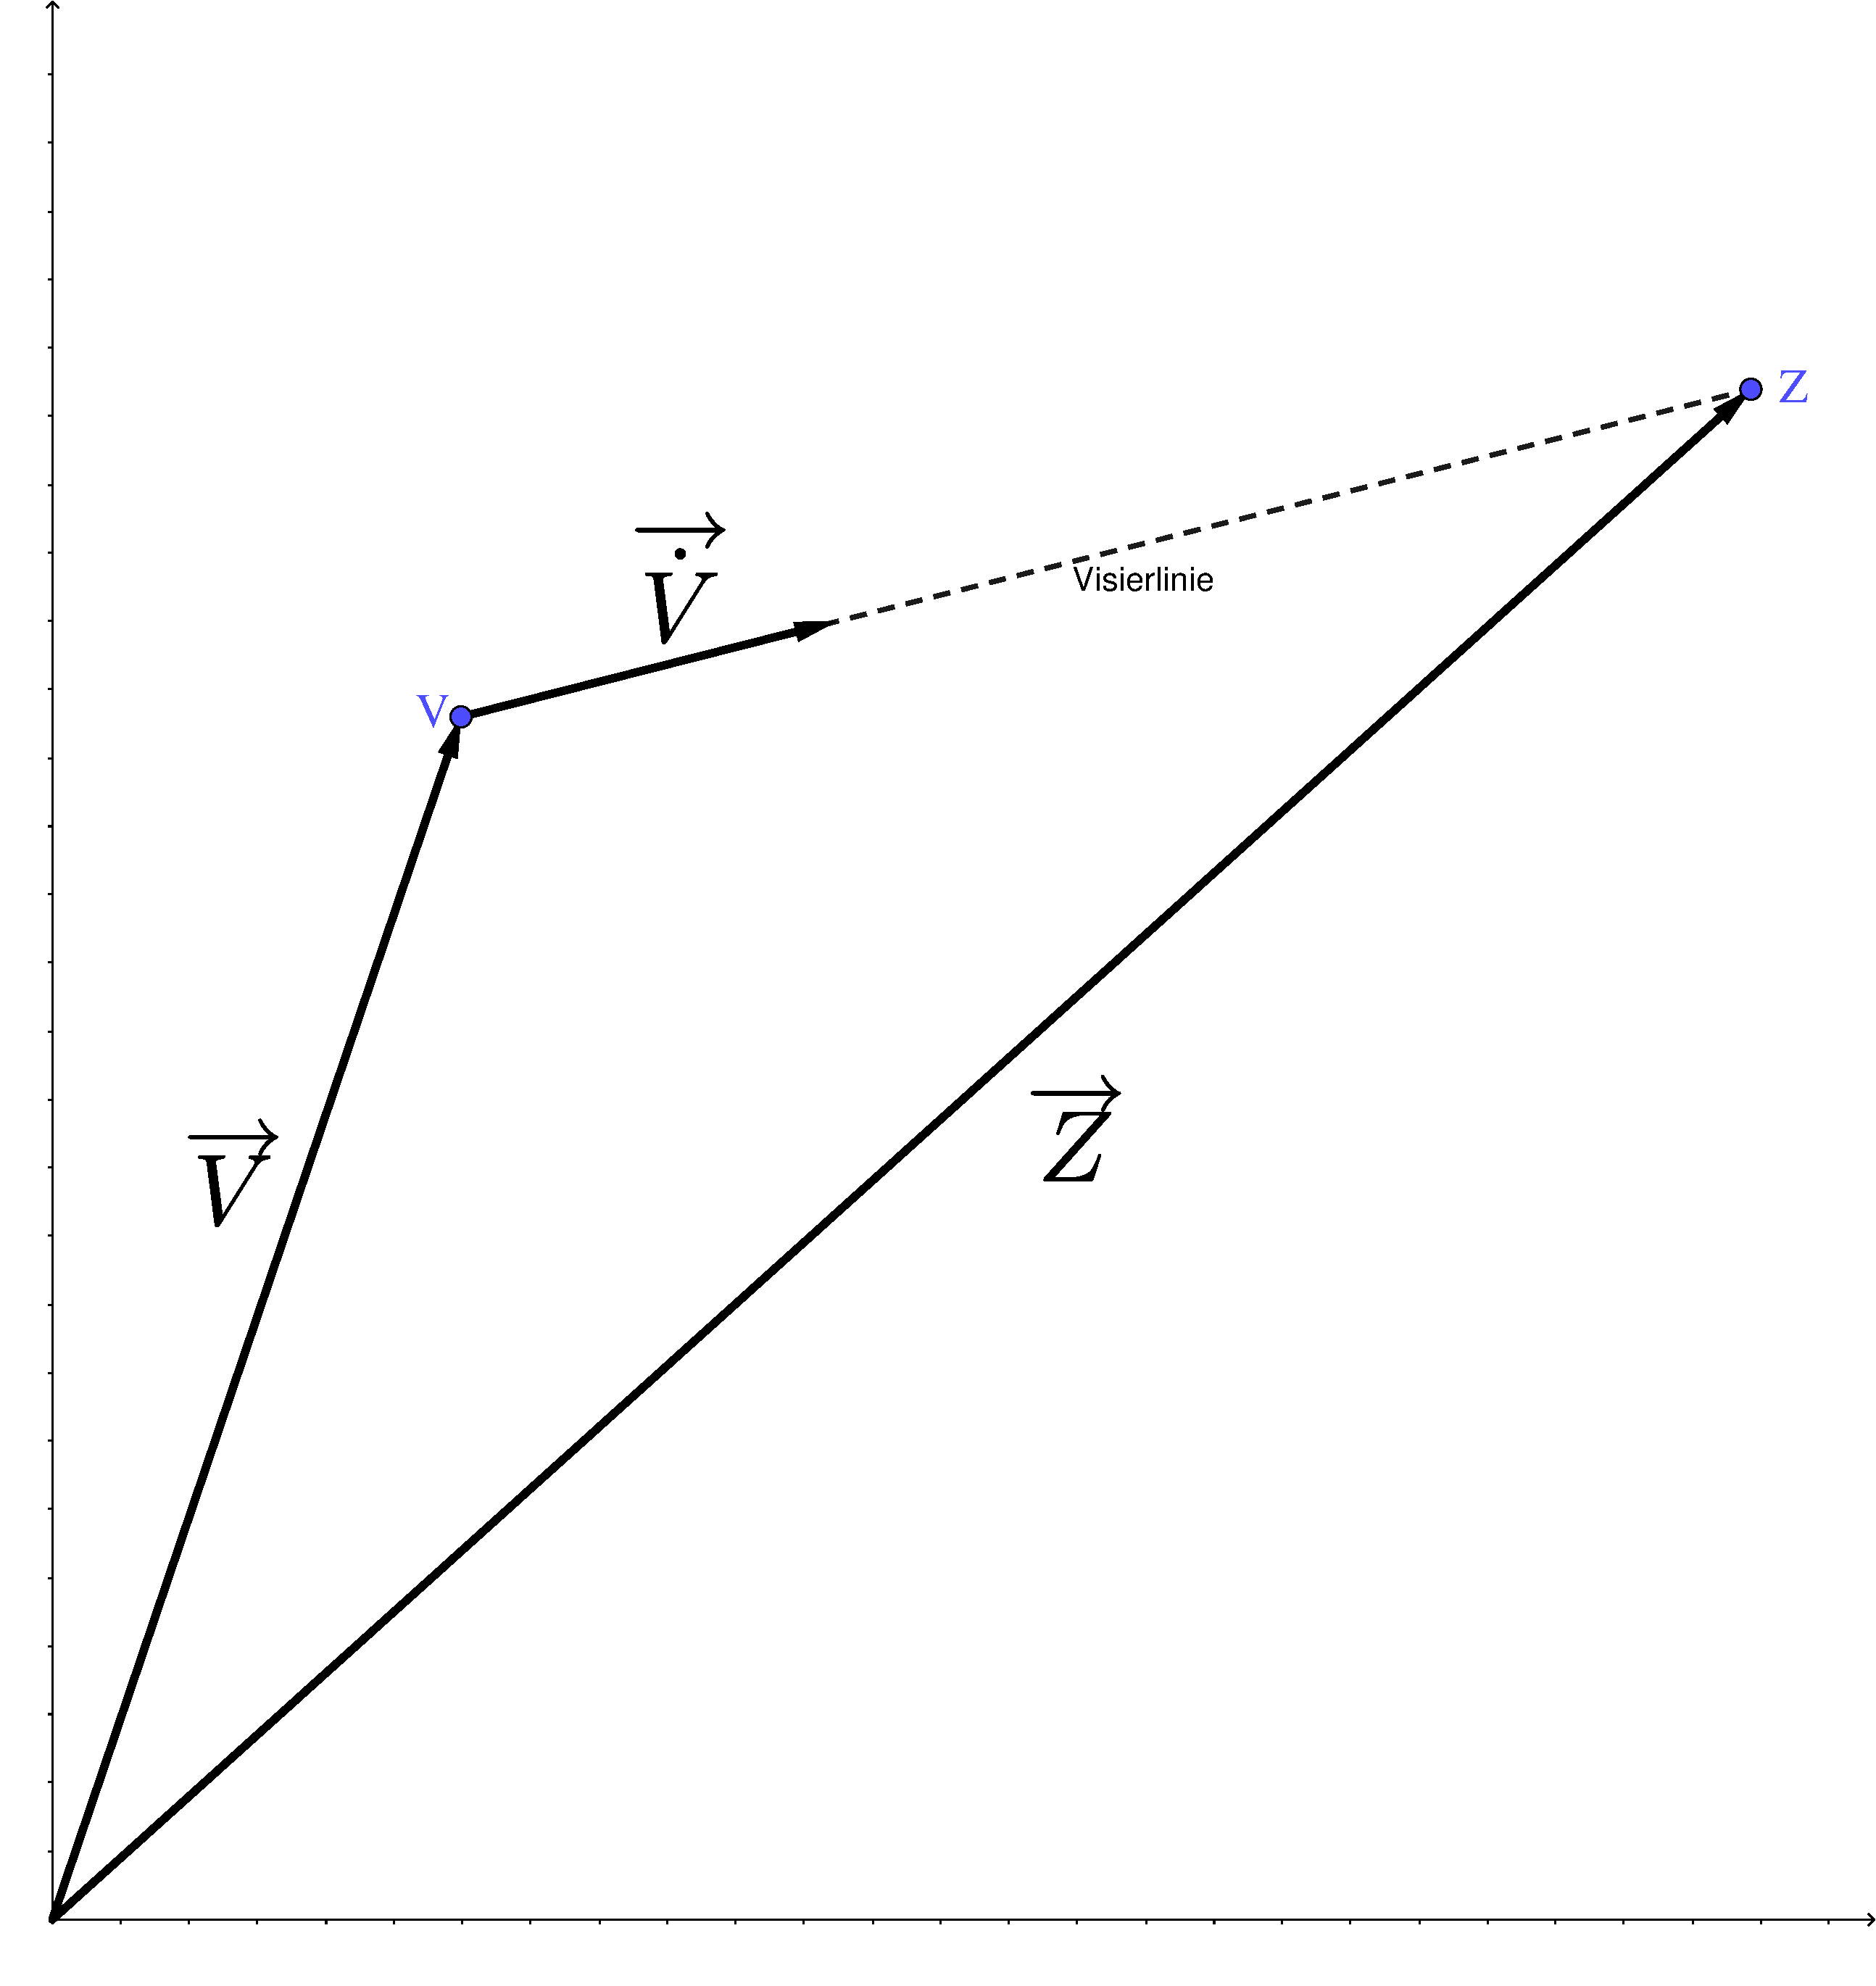
\includegraphics{.\papers\lambertw\Bilder\pursuerDGL2.pdf}
%    \label{pursuer:pursuerDGL2}
%\end{figure}

In der Tabelle \eqref{lambertw:Strategien} sind drei mögliche Strategien aufgezählt.
Folgend wird nur noch auf die Strategie 1 eingegangen.
Bei dieser Strategie ist die Geschwindigkeit konstant und der Verfolger bewegt sich immer direkt auf sein Ziel hinzu.
In der Grafik \eqref{lambertw:pursuerDGL2} ist das Problem dargestellt.
Wobei $\overrightarrow{V}$ der Ortsvektor des Verfolgers, $\overrightarrow{Z}$ der Ortsvektor des Ziels und $\overrightarrow{\dot{V}}$ der Geschwindigkeitsvektor des Verfolgers ist.
Die konstante Geschwindigkeit kann man mit der Gleichung
\begin{equation}
    |\overrightarrow{\dot{V}}|
    = konst = A
    \quad|A\in\mathbb{R}>0
\end{equation}
darstellen. Der Geschwindigkeitsvektor wiederum kann mit der Gleichung
\begin{equation}
    \frac{\overrightarrow{Z}-\overrightarrow{V}}{|\overrightarrow{Z}-\overrightarrow{V}|}\cdot|\overrightarrow{\dot{V}}|
    =
    \overrightarrow{\dot{V}}
\end{equation}
beschrieben werden.
Durch die Subtraktion der Ortsvektoren $\overrightarrow{V}$ und $\overrightarrow{Z}$ entsteht ein Vektor der vom Punkt $V$ auf $Z$ zeigt.
Da die Länge dieses Vektors beliebig sein kann, wird durch Division mit dem Betrag, die Länge auf eins festgelegt.
Aus dem Verfolgungsproblem ist auch ersichtlich, dass die Punkte $V$ und $Z$ nicht am gleichen Ort starten und so eine Division durch Null ausgeschlossen ist.
Wenn die Punkte $V$ und $Z$ trotzdem am gleichen Ort starten, ist die Lösung trivial.
Nun wird die Gleichung mit deren rechten Seite skalar multipliziert, um das Gleichungssystem von zwei auf eine Gleichung zu reduzieren.
\begin{align}
    \label{pursuer:pursuerDGL}
    \frac{\overrightarrow{Z}-\overrightarrow{V}}{|\overrightarrow{Z}-\overrightarrow{V}|}\cdot
    \overrightarrow{\dot{V}}
    &=
    |\overrightarrow{\dot{V}}|^2
    \\
    \frac{\overrightarrow{Z}-\overrightarrow{V}}{|\overrightarrow{Z}-\overrightarrow{V}|}\cdot \frac{\overrightarrow{\dot{V}}}{|\overrightarrow{\dot{V}}|}
    &=
    1
\end{align}
Diese DGL ist der Kern des Verfolgungsproblems, insofern der Verfolger die Strategie 1 verwendet.


\subsection{Ziel
\label{lambertw:subsection:Ziel}}
Als nächstes gehen wir auf das Ziel ein.
Wie der Verfolger wird auch unser Ziel sich strikt an eine Fluchtstrategie halten, welche von Anfang an bekannt ist.
Diese Strategie kann als Parameterdarstellung der Position nach der Zeit beschrieben werden.
Zum Beispiel könnte ein Ziel auf einer Geraden flüchten, welches auf einer Ebene mit der Parametrisierung
\begin{equation}
    \vec{r}(t)
    =
    \begin{Bmatrix}
        0\\
        t
    \end{Bmatrix}
\end{equation}
beschrieben werden könnte.
Mit dieser Gleichung ist das Ziel auch schon vollumfänglich definiert.
Die Fluchtkurve kann eine beliebige Form haben, jedoch wird die zu lösende DGL immer komplexer.




